\chapter{Applied cryptography}
\lecture{2}{14/10}

\section{Basic encryption}

\begin{definition}[Cryptography]
    \textbf{Cryptograph} is the study of techniques for secure communication in the presence of adversaries.
\end{definition}

\begin{example}[Encryption]
    The following is an example of encryption by using a \textbf{cipher}.
    \begin{center}
        \begin{tabular}{ccccc}
            Hello, World! & $\underset{\text{encryption}}{\implies}$ & Baqqj, Pjsqx! & $\underset{\text{decryption}}{\implies}$ & Hello, World!
        \end{tabular}
    \end{center}
\end{example}

\begin{definition}[Substitution cipher]
    A \textbf{substitution cipher} is an encryption technique in which units in plaintext are converted to ciphertext.
\end{definition}

\begin{example}[ROT13]
    An example of a substitution cipher is \emph{ROT13}, where each letter is replaced with the letter 13 places down from it. This can be generalised to ROT-$k$, where we replace a letter with the letter $k$ places away from it. Obviously, ROT-$k$ is easy to break as for a plaintext using an alphabet $\Sigma$, there is only $\lvert \Sigma \rvert - 1$ different ROT ciphers we need to test, and decrypting ROT is very easy. An example of the bijection used in ROT13 is shown in Figure \ref{fig:rot13}.
\end{example}

\begin{figure}
    \centering
    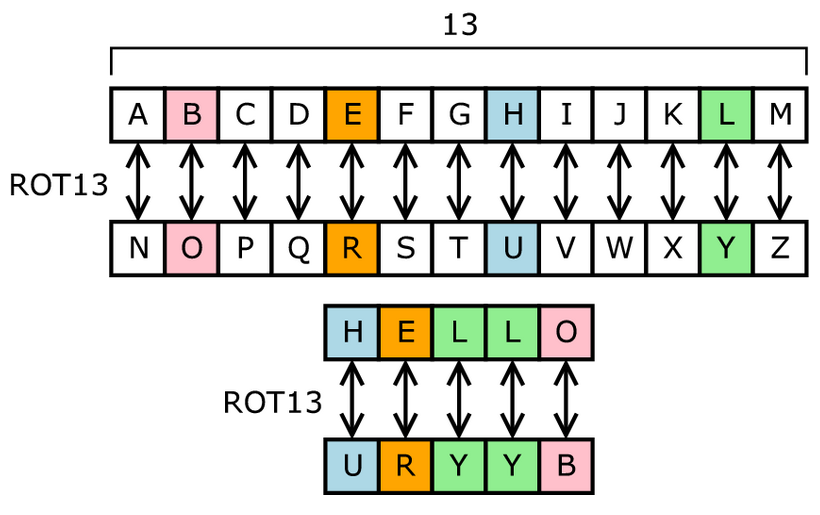
\includegraphics[width=0.8\linewidth]{images/rot13.png}
    \caption{ROT13 bijection with example.}
    \label{fig:rot13}
\end{figure}

\begin{example}[Variations of substitution cipher]
    Our definition for a substitution cipher was purposely vague, we can many different variations of it:
    \begin{enumerate}
        \item monoalphabetic: fixed substitutions for the entire text;
        \item polyalphabetic: change substitution rules throughout the text; and
        \item polygraphic: substitute with groups of letters instead of individual letters.
    \end{enumerate}
    You may be able to see that polygraphic ciphers drastically improve the effectiveness of the encryption as it squares the nunmber of combinations. 
\end{example}

\begin{remark}
    There has been a lot of variations of ciphers used in encryption throughout time; however, they are not often used anymore as they are easy to break via divide-and-conquer approaches. In pracitse, we typically use \textbf{keys} to encrypt messages.
\end{remark}

\begin{definition}[Key]
    A \textbf{key} is a parameter to a cryptographic algorithm.
\end{definition}

This is a very vague but effective definition. Our cryptographic algorithm will take our message and a key and then encrypt it into \textbf{ciphertext}.

\begin{definition}[Symmetric-key and asymmetric-key algorithms]
    We say an encryption algorithm is \textbf{symmetric} if the same key is used to encrypt plaintext and decrypt ciphertext. If different keys are used, then the algorithm is \textbf{asymmetric}.
\end{definition}

\begin{example}[SSH]
    \textbf{Secure Shell} (SSH) is a cryptographic network protocol that uses public-key cryptography (also called asymmetric). So when data wants to be transferred between two hosts, the host establishing the connection will generate a public key for encryption and a private key for decryption. The host will hand out the public key for hosts to encrypt then send their data, and the private key (which is kept secure) is used to decrypt it.
\end{example}

\begin{example}[Block cipher]
    \textbf{Block ciphers} are symmetric algorithms that are typically used to encrypt files. They encrypt blocks of text at a time using a symmetric key and are deterministic. The reason for it being deterministic is to avoid encrypting the same block of data twice. \textbf{Initialisation vectors} are fixed-size inputs that are used to be random (a crucial property for encryption).
\end{example}

\begin{definition}[Side-channel attack]
    A \textbf{side-channel attack} is an attack on a system that exploits the physical implementation of a system as opposed to vulnerabilities in the implemented algorithms. Measureable values such as power consumption and electromagnetic leakage can be exploited for information.
\end{definition}

\section{Hashing}

Storing passwords in plaintext is a terrible idea; if someone gains access to the database then all users are exposed. This is why hashes exist.

\begin{definition}[Hash function]
    A \textbf{hash function} $f$ maps data of arbitrary size on to a fixed size. We evaluate the effectiveness of a hashing algorithm by the following properties:
    \begin{enumerate}
        \item deterministic;
        \item one-way function (not easily invertable);
        \item no collisions; and
        \item avalance effect (a small change in input causes a significant change in output).
    \end{enumerate}
\end{definition}

\begin{example}[Examples of hash functions]
    Some examples of hash functions include
    \begin{enumerate}
        \item MD5, deemed too insecure;
        \item SHA-1, deemed too insecure; and
        \item SHA-2, not deemed insecure but vulnerable to certain attacks.
    \end{enumerate}
\end{example}

\begin{example}[Breaking MD5]
    If we assume that a password $p \in \Sigma^8$ where $\lvert \Sigma \rvert = 94$, then there are $94^8 \approx 6 \times 10^{15}$ different possibilities of passwords. Assuming we can check $10^{10}$ hashes per second, this would take about 7 days to crack any password. We refer to this type of attack, where we have access to the encrypted material, as a \textbf{offline attack}.
\end{example}

\begin{definition}[Rainbow table]
    A \textbf{rainbow table} is a pre-computed table for reversing cryptographic hash functions. They typically store every plaintext password and the associated hash, so if you can find someone's password given a hash.
\end{definition}

\begin{remark}
    We can sort rainbow tables by the hash, then searching this list with our hash is going to be a much less intensive operations then calculating hashes. Rainbow tables are a good example of a \textbf{space-time tradeoff}.
\end{remark}

So if we have a table of all passwords and their respective hashes, how do we stop against these types of attacks? \textbf{Salt}.

\begin{definition}[Salt]
    A \textbf{salt} is a piece of random data that is added to a one-way hashing function (typically) to help safeguard storage (of passwords).
\end{definition}

\begin{remark}
    Using salts now take away from the deterministic nature of a hashing algorithm, kind of. The hashing algorithm will still give the same result if you give it the same input and salt, but as the salt is randomised every time two users with the same password will have different hashes. When a salt value is generated from a password, both the salt and the hash is stored.
\end{remark}
